\documentclass{article}
\usepackage[utf8]{inputenc}
\usepackage{geometry}
\usepackage{amsmath}
\usepackage{amssymb}
\usepackage{amsfonts}
\usepackage{graphicx}
\usepackage[thmmarks, amsmath, thref]{ntheorem}
\usepackage{times} % Fuente Times New Roman
\geometry{a4paper, left=2cm, right=2cm, top=1cm, bottom=1.5cm}
\setlength{\parskip}{0pt} % Espaciado compacto
\setlength{\parindent}{0em}

% Configuración del entorno "Solución"
\theoremstyle{nonumberplain}
\theoremheaderfont{\itshape}
\theorembodyfont{\upshape}
\theoremseparator{.}
\theoremsymbol{\ensuremath{\square}}
\newtheorem{solucion}{Solución}

\begin{document}

\textbf{Problema:} 
a) Use el Teorema de la Función Inversa para encontrar la función inversa de \( f(x, y) = (x+3y, x-2y) \) cerca del punto \( (1,0) \).  
b) Dibuje un diagrama de árbol y formule la Regla de la Cadena para \( \frac{\partial w}{\partial s} \) con \( w=f(x, y) \), \( x=g(r, s, t) \), y \( y=h(r, s, t) \). \\

\begin{solucion}
**Parte a: Encontrar la función inversa** \\

La función \( f(x, y) = (x+3y, x-2y) \) se define como:
\[
   \begin{cases}
   u = x + 3y \\
   v = x - 2y
   \end{cases}
\]
Resolviendo este sistema de ecuaciones para \( x \) y \( y \):
\[
u - v = (x + 3y) - (x - 2y) = 5y \quad \Rightarrow \quad y = \frac{u - v}{5}
\]
Sustituyendo \( y \) en \( u = x + 3y \):
\[
u = x + 3\left(\frac{u - v}{5}\right) \quad \Rightarrow \quad u = x + \frac{3u - 3v}{5} \\
5u = 5x + 3u - 3v \quad \Rightarrow \quad 2u + 3v = 5x \quad \Rightarrow \quad x = \frac{2u + 3v}{5}
\]
Por lo tanto, la función inversa es:
\[
f^{-1}(u, v) = \left( \frac{2u + 3v}{5}, \frac{u - v}{5} \right)
\]

**Parte b: Regla de la Cadena** \\

Considere \( w = f(x, y) \), donde \( x = g(r, s, t) \) y \( y = h(r, s, t) \). Según la regla de la cadena, la derivada parcial de \( w \) respecto a \( s \) se escribe como:
\[
\frac{\partial w}{\partial s} = \frac{\partial f}{\partial x} \cdot \frac{\partial x}{\partial s} + \frac{\partial f}{\partial y} \cdot \frac{\partial y}{\partial s}
\]
Esto se justifica porque \( w \) depende indirectamente de \( s \) a través de \( x \) y \( y \). La variación de \( w \) respecto a \( s \) incluye:
\begin{enumerate}
    \item El cambio en \( w \) debido a \( x \), ponderado por cómo cambia \( x \) con \( s \).
    \item El cambio en \( w \) debido a \( y \), ponderado por cómo cambia \( y \) con \( s \).
\end{enumerate}

**Diagrama de árbol:**  
\begin{figure}[h]
    \centering
    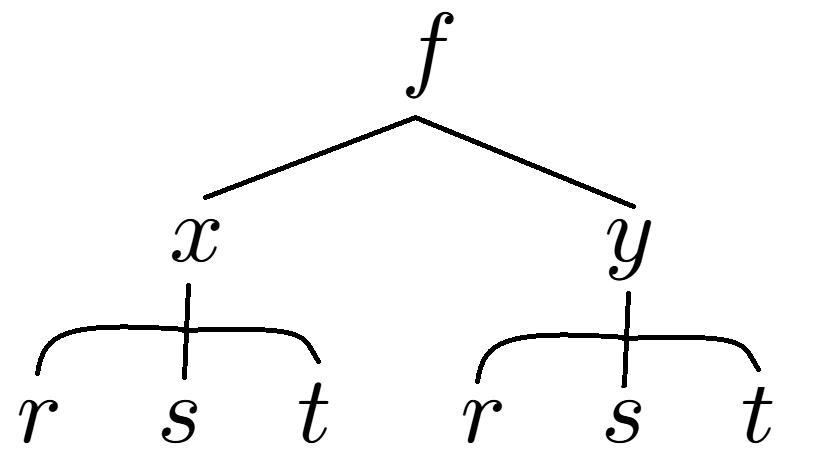
\includegraphics[width=0.4\linewidth]{Diagram.png}
    \caption{Diagrama de árbol mostrando las dependencias de \( w \) respecto a \( s \) por composición.}
    \label{fig:tree-diagram}
\end{figure}

El diagrama muestra cómo \( w \) depende de \( x \) e \( y \), que a su vez dependen de \( r, s, t \).

\end{solucion}

\end{document}
